% Please use the skeleton file you have received in the
% invitation-to-submit email, where your data are already
% filled in. Otherwise please make sure you insert your
% data according to the instructions in PoSauthmanual.pdf
\documentclass{PoS}

\usepackage{amsmath}
\usepackage{xspace}   % decides whether to insert a space or not
\usepackage{fixmath}
\usepackage{bm,braket}
\usepackage[mathcal]{euscript}
\usepackage{wrapfig}

% Definitions
\newcommand{\calB}{\mathcal B}
\newcommand{\calS}{\mathcal S}
\newcommand{\calH}{\mathcal H}
\newcommand{\order}[1]{{{\cal O}\left(#1\right)}}
\newcommand{\ttbar}{\ensuremath{t \bar t}\xspace}
\newcommand{\qqbar}{\ensuremath{q \bar q}\xspace}
\newcommand{\qbar}{\ensuremath{\bar q}\xspace}
\newcommand{\bfw}{\bm{w}}
\newcommand{\gammaE}{\gamma_E}
\newcommand{\ie}{{\it i.e. }}
\newcommand{\comment}[1]{\textbf{\color{red}[#1]}}
\newcommand{\LT}{L_\perp}
\newcommand{\iibar}{{i \bar i}}
\newcommand{\bfS}{\bm{S}}
\newcommand{\tbfS}{{\tilde \bfS}}
\newcommand{\bfgamma}{\bm{\gamma}}
\newcommand{\bfI}{\bm{1}}
\newcommand{\bfGamma}{\bm{\Gamma}}
\newcommand{\bfZ}{\bm{Z}}
\newcommand{\bare}{\text{bare}}

\title{Top pair production at NNLO}

\ShortTitle{Top pair production at NNLO}

\author{\speaker{Sebastian Sapeta}\thanks{
  Based on work done in collaboration with Micha\l{} Czakon and Ren\'e
  \'Angeles-Mart\'inez.
  }\\
  %
  Institute of Nuclear Physics, Polish Academy of Sciences \\
  ul.\ Radzikowskiego 152, 31-342 Krak\'ow, Poland\\
  %
  E-mail: \email{sebastian.sapeta@ifj.edu.pl}}

\abstract{
We report on progress towards calculating the NNLO cross section for top quark
pair production in the the framework which combines the $q_T$-slicing method and
small-$q_T$ factorization. 
%
In this contribution, we present the complete result for the small-$q_T$ soft
function at NNLO, which constitutes the main challenge on the way to our
goal.
%
In order to evaluate the divergent integrals appearing in the calculation, we
develop methods based on sector decomposition and differential equations. We
present complete validation of our framework and provide results which are
ready for application in the calculation of the $t\bar t$ cross section at
NNLO.

}


\FullConference{Loops and Legs in Quantum Field Theory (LL2018)\\
                29 April 2018 - 04 May 2018\\
		St. Goar, Germany}

\begin{document}

%-----------------------------------------------------------------------------
\section{Introduction}

The increasing accuracy of experimental data coming from the LHC is in many
cases superior to that of theoretical predictions. 
%
If it comes to corrections from Quantum Chromodynamics, 
the state of the art for most processes of interest has 
recently changed from NLO to NNLO. Some gaps still need to be filled, however,
and additional work is required to fully test the NNLO results and implement
them in efficient public codes such that they can benefit experimental analyses.
%
At the same time, the calculation of the N$^3$LO cross section for the
Higgs boson production from gluon fusion~\cite{Anastasiou:2015ema} has marked
the first step on the way towards pushing the accuracy of QCD predictions to the
next level.

One of the most important class of measurements studied at the LHC are processes
which involve production of the top quark. And, in particular, top-anti-top
production, which is relevant both in studies of properties of the Standard
Model, as well as in searches for new physics, as it forms significant
backgrounds to many signatures. The cross section for this process is currently
known up to NNLO~\cite{Baernreuther:2012ws, Czakon:2012pz, Czakon:2012zr,
Czakon:2013goa, Czakon:2015owf, Czakon:2016ckf}.

In this proceedings, we present the calculation of the complete, small-$q_T$
NNLO soft function for top quark pair production. 
%
This result, together with the framework and tools developed to obtain it, form
key  elements of an alternative calculation of the complete NNLO cross section
for that process.

The motivation behind our work is two-fold. On one hand, it will lead to a
second, independent result for the NNLO top pair production cross section,
which, given the complexity of the calculation, is highly desirable.
At the same time, our work forms a stepping stone towards developing a general
framework for calculations of N$^3$LO QCD corrections to a wide range of
processes of relevance for hadron colliders.


%-----------------------------------------------------------------------------
\section{Theoretical framework}

The approach for achieving NNLO accuracy for the top pair production,
presented in this proceedings, is part of a wider strategy for calculating
N$^m$LO contributions to processes of the type
%
\begin{equation}
  h_1 + h_2 \to F\, {\textstyle (q_T)} + X\,,
  %\label{eq:}
\end{equation}
%
where two hadrons, $h_1$ and $h_2$, collide and produce an object $F$, which is
registered in a detector, together with an undetected QCD radiation $X$. 
%
Our framework is suitable both when $F$, whose transverse momentum is denoted by
$q_T$, is a colour-neutral object (single EW boson, pair of EW bosons, the
Higgs), as well as when it carries colour, like in the case of the top quark
pair. 

If we choose to use the $q_T$-slicing method, we are able to write the cross
section as
a sum of two components~\cite{Catani:2007vq, Bonciani:2015sha}
%
\begin{equation}
  \frac{\sigma_{{\rm N}^m{\rm LO}}^{F}}{d\Phi} = 
  %\sigma_{{\rm N}^m{\rm LO}}^{F} = 
  \int^{q_{T{\rm cut}}}_0 
  \!\!\!\!\! d q_T\,
  \frac{d\sigma^{F}_{{\rm N}^m{\rm LO}}}{d\Phi dq_T} +
  \int_{q_{T{\rm cut}}}^\infty 
  \!\!\!\!\! d q_T\,
  \frac{d\sigma^{F + {\rm jet}}_{{\rm N}^{m-1}{\rm LO}}}{d\Phi dq_T}\,,
  \label{eq:qT-slicing}
\end{equation}
%
each of which is separately finite.
%
The advantage of this approach is that the second term in the above equation,
which represents resolved emissions, is required only at the N$^{m-1}$LO
accuracy, and it is already known in most relevant cases.  
%
On the contrary, the first term in Eq.~(\ref{eq:qT-slicing}), which combines
virtual and unresolved real corrections, is usually unknown. However it is
needed only in the small-$q_T$ approximation.

In order to calculate the latter we use the Soft Collinear Effective
Theory~(SCET)~\cite{Becher:2014oda}, in which the cross section factorizes at
small $q_T$ according to the formula
%
\begin{equation}
  \frac{d\sigma^F_{{\rm N}^m{\rm LO}}}{d\Phi dq_T} = 
  \calB_1^{{\rm N}^m{\rm LO}}\otimes
  \calB_2^{{\rm N}^m{\rm LO}}\otimes
  \calH^{{\rm N}^m{\rm LO}}\otimes
  \calS^{{\rm N}^m{\rm LO}} +
  \order{\frac{q_T^2}{q^2}} \,,
  \label{eq:smallqT-cs}
\end{equation}
%
where $q^2$ is the invariant mass of the object $F$.
%
The functions appearing in the above equation account for contributions coming
from different phase space regions of $X$. Specifically, the beam functions
$\calB_i$ sum up emissions of collinear and anti-collinear partons, the hard
functions, $\calH$, accounts for hard radiation, and the soft function, $\calS$,
sums emissions from soft, real gluons.
%
The calculation of each of these functions is considerably simpler than the
calculation of the complete cross section. In addition, some of the functions
are already available from the literature.

In the case of the top quark pair production, the beam functions are known up to
NNLO~\cite{Gehrmann:2012ze,Gehrmann:2014yya} and the NNLO hard function can be
extracted from Refs.~\cite{Czakon:2008zk, Baernreuther:2013caa}. However, the
small-$q_T$ soft function is only known up to NLO~\cite{Li:2013mia,
Catani:2014qha}. Hence, in order to achieve the NNLO accuracy of the \ttbar
cross section, one needs to calculate the missing NNLO correction to the soft
function appearing in Eq.~(\ref{eq:smallqT-cs}) (We note that such calculation
shares many features with that of the NNLO soft function for top pair production
in the threshold limit~\cite{Ferroglia:2012uy, Wang:2018vgu}. However, the
result for the latter is not of direct use in our context.)

The soft function for our process of interest can be schematically defined with
the following equation
%
\begin{equation}
  {\textstyle S^\text{bare}(q_T,\beta,\theta) } = \sum 
  \!\!\!\! \!\!
  \vcenter{\hbox{
  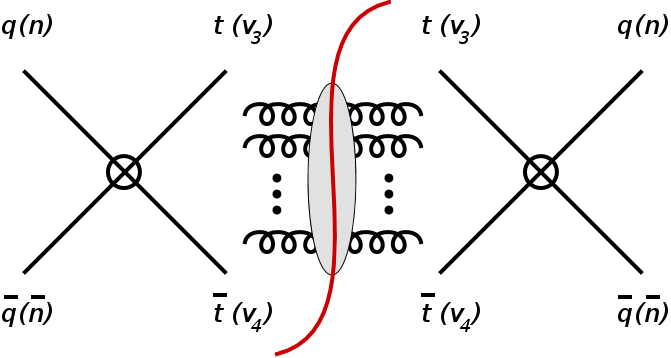
\includegraphics[width=0.39\textwidth]{plots/sf-schematic.png}}}
  {\textstyle \delta\left(q_T - \left|\sum_i k_{i\perp} \right|\right)
  \prod_i \delta^{+}(k_i^2) }\,.
  \label{eq:sf-all-orders}
\end{equation}
%
To this end, we focus on the $\qqbar \to \ttbar$ subprocess and introduce the
following notation for the 4-momenta: 
$p_q = m_t n$, $p_{\bar q} = m_t \bar n$ and 
$p_t = m_t v_3 + l_3$, $p_{\bar t} = m_t v_4 + l_4$, where 
$n = (1,0,0,1)$, $\bar n = (1,0,0,-1)$. 
%
We see that in the definition~(\ref{eq:sf-all-orders}), the transverse
momenta of real emissions are restricted to sum up to a fixed value of $q_T$.
Because the gluons are soft, $l_i \ll m_t v_i$, and the velocities satisfy Born
kinematics, $n+\bar n = v_3 + v_4$, at each perturbative order. Apart from
$q_T$, the soft function of Eq.~(\ref{eq:sf-all-orders}) depends on $\beta =
\sqrt{1-4m_t^2/q^2}$ and $\theta$, where the latter is the scattering angle of
the top quark in the \ttbar rest frame.

The NNLO soft function corresponds to a sum of all $\order{\alpha_s^2}$
contributions from Eq.~(\ref{eq:sf-all-orders}). They take forms of
$2d$-dimensional integrals which exhibit soft and rapidity singularities. The
latter arise when the light-cone components of the gluon 4-momenta become very
small or very large, and are not removed by dimensional regularization. 
%
In our
calculation, we adopt the prescription of Ref.~\cite{Becher:2011dz} which turns
the above divergences into poles in a new regulator $\alpha$. Even though the
individual integrals suffer from rapidity divergences, their complete sum, hence
the soft function, is finite in the limit $\alpha \to 0$~\cite{Li:2013mia,
Becher:2011dz}.

Each function defined on the right hand side of Eq.~(\ref{eq:smallqT-cs}), when
calculated directly from diagrammatic definitions, like the one given in
Eq.~(\ref{eq:sf-all-orders}) for the soft function, is separately divergent.
These divergencies correspond to soft and collinear limits and they must cancel
between the hard, soft and beam functions, as the entire cross section has to be
finite. 

It turns out to be useful to remove divergences also at the level of the
functions entering the factorization formula~(\ref{eq:smallqT-cs}). This can be
achieved by the procedure of multiplicative renormalization. For example, the
renormalized soft function is given by
%
\begin{equation}
  \bfS(\mu) = \bfZ^\dagger_s(\mu,\epsilon) \bfS^\bare(\epsilon)
  \bfZ_s(\mu,\epsilon)\,,
  \label{eq:Srendef}
\end{equation}
%
where the coefficient $\bfZ_s(\mu,\epsilon)$ absorbs all soft divergences such
that $\bfS(\mu)$ is finite.

As usual in the procedure of renormalization, the renormalized object acquires
dependence on an arbitrary parameter $\mu$, which has to vanish at the level of
the cross section. This implies that the renormalized soft function of
small-$q_T$ factorization must satisfy the following RGE
equation~\cite{Zhu:2012ts}
%
\begin{equation}
  \frac{d}{d\ln \mu} \bfS_\iibar (\mu) =
  - \bfgamma^{s \dagger}_\iibar \,\bfS_\iibar (\mu)  
  - \bfS_\iibar (\mu)\, \bfgamma^{s}_\iibar \,,
  \label{eq:SF-RGE-main}
\end{equation}
%
where
%
\begin{equation}
  \bfgamma^{s}_\iibar = \bfgamma^{h}_\iibar - 2 \gamma^{i} \bfI\,,
  %\label{eq:}
\end{equation}
%
and $\bfgamma^{h}_\iibar$ is defined as a non-$\Gamma_\text{cusp}$ part of the
full anomalous dimension matrix $\bfGamma$~\cite{Ahrens:2010zv}, while
$\gamma^{i}$ is the massless-particle anomalous dimension (and enters RGE
equations for beam functions in Drell-Yan and Higgs
production~\cite{Becher:2010tm, Becher:2012yn}). 
%
The soft anomalous dimension matrix $\bfgamma^{s}$ is related to the soft
renormalization factor (also a matrix in colour space), $\bfZ_s$, as follows
%
\begin{equation}
  \bfgamma^{s} = - \bfZ_s^{-1}\frac{d\bfZ_s}{d\ln \mu}\,.
  %\label{eq:}
\end{equation}

Each quantity in Eq.~(\ref{eq:Srendef}) has a perturbative expansion in 
the strong coupling $\alpha_s$. This allows one to relate the bare and
renormalized objects order by order. At NNLO, the renormalized soft function
is given by
%
\begin{equation}
  \bfS^{(2)}_\text{ren} = 
  \bfZ^{\dagger (2)}_s \bfS^{(0)}_\bare  + 
  \bfS^{(0)}_\bare \bfZ^{(2)}_s  +
  \bfZ^{\dagger (1)}_s \bfS^{(0)}_\bare \bfZ^{(1)}_s 
  +
  \bfZ^{\dagger (1)}_s \bfS^{(1)}_\bare  + 
  \bfS^{(1)}_\bare \bfZ^{(1)}_s  +
  \bfS^{(2)}_\bare
  -\frac{\beta_0}{\epsilon}\, \bfS^{(1)}_\bare \,.
  \label{eq:renS2}
\end{equation}
%
The quantity on the left hand side is finite, while the objects on the right
hand side exhibit divergencies in the soft limit. These divergencies are
dimensionally regularized (in the $\overline{\text{MS}}$ scheme) and they
correspond to poles in $\epsilon$. The first three terms on the right hand side
of Eq.~(\ref{eq:renS2}) contain the pole part only, while other terms have both
finite and pole parts. The poles of the bare soft function, $\bfS^{(2)}_\bare$,
which we obtain through direct calculation following the definition of
Eq.~(\ref{eq:sf-all-orders}), should match the poles from the other terms on the
right hand side of Eq.~(\ref{eq:renS2}), which can be determined from the
renormalization group. The cancellation of $\epsilon$ poles provides a strong
cross check which we will use as part of the validation of our framework.


%-----------------------------------------------------------------------------
\section{NNLO soft function: methods of calculation}

\begin{figure}[t]
  \begin{center}
    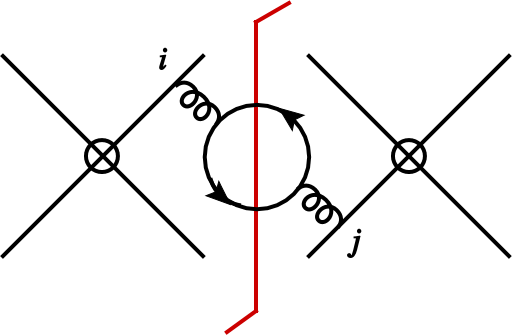
\includegraphics[width=0.30\textwidth]{plots/sf-nnlo-nf.png}
    \hfill
    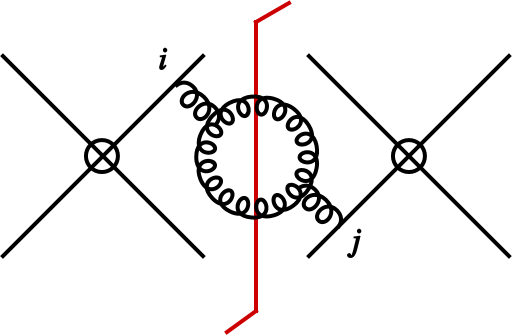
\includegraphics[width=0.30\textwidth]{plots/sf-nnlo-gluon.png}
    \hfill
    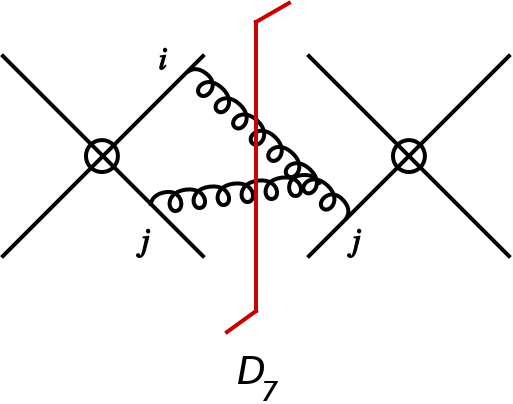
\includegraphics[width=0.30\textwidth, trim ={0 65pt 0 0}, clip]{plots/sf-nnlo-3gv.png}
    \hfill
    \vspace{20pt}
    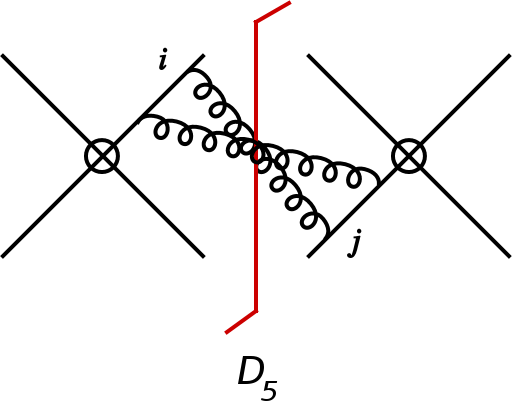
\includegraphics[width=0.30\textwidth, trim ={0 65pt 0 0}, clip]{plots/sf-nnlo-d5.png}
    \hfill
    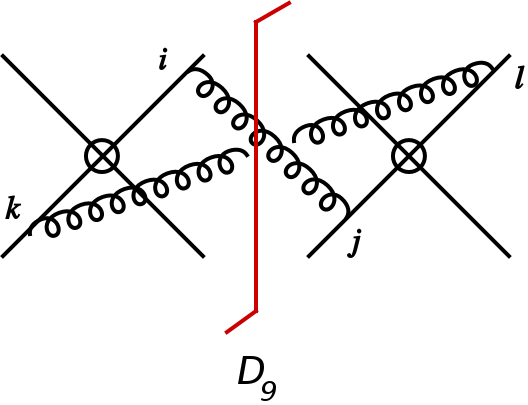
\includegraphics[width=0.30\textwidth, trim ={0 65pt 0 0}, clip]{plots/sf-nnlo-4wl.png}
    \hfill
    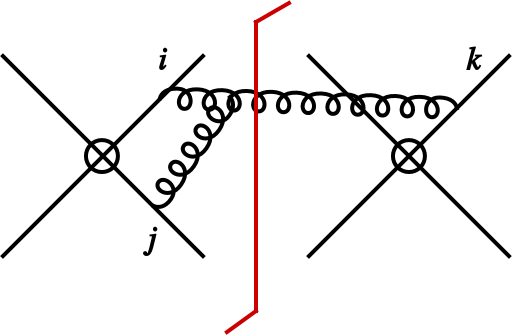
\includegraphics[width=0.30\textwidth]{plots/sf-nnlo-real-virtual1.png}
  \end{center}
  \caption{
    Example diagrams contributing to the NNLO soft function for top pair
    production.
  }
  \label{fig:example-sf-diagrams}
\end{figure}

The soft function at NNLO receives contributions from several classes of
diagrams. The complete formula can be schematically written as
%
\begin{equation}
  S^{(2)}_\text{bare} = 
  S_\text{2-cut, $q\bar q$} + 
  S_\text{2-cut, $gg$} + 
  S_\text{1-cut} + 
  S_\text{0-cut}\,.
  \label{eq:SFbare-contr}
\end{equation}
%
Example diagrams are given in Fig.~\ref{fig:example-sf-diagrams}. They include
quark bubble, gluon bubble, abelian and non-abelian graphs. We also notice
that gluons can connect different numbers of  distinct Wilson lines: two, three
or four.

We apply different methods of calculation to different classes of integrals. The
bubble diagrams, as well as parts of the non-abelian, three-Wilson line,
double-cut graphs, which we call ``tadpole'', are calculated almost entirely
analytically with help of the method of differential equations. Single-cut
integrals are calculated directly by a combination of analytic and numerical
methods. The remaining integrals, namely those coming from double-cut,
non-tadpole diagrams, are computed with the method of sector decomposition,
adapted to our specific problem. This set of integrals poses the most difficult
challenge in our calculation.  

With an exception of the propagators introduced to regularize rapidity
divergences, the bubble diagrams depend only on the momenta $k$ and $k+l$. This
feature allows one to first integrate them over $k+l$, a generalization of
the standard vacuum polarization tensor calculation, and then solve the integral
over $k$ with the method of differential equations.

Since the gluons connected to the Wilson lines are not cut in the bubble
diagrams,  the integrals involve a function of $\theta(k^2)$. In our calculation
we trade it for the Dirac delta function at the cost of introducing an extra
integral over the mass by applying the identity $1 = \int_0^\infty dm^2
\delta(k^2-m^2)$. This allows us then to use reverse unitarity and turn all
delta functions into propagators. We obtain a topology which consists of
six propagators. 
%
All the integrals needed for the bubble diagrams can be reduced to five master
integrals for which we then derive a set of differential equations with respect
to the variable~$\beta$. For reduction, we used our private C++ implementation of
the Laporta algorithm~\cite{Laporta:2001dd}, which depends on {
FORM}~\cite{Ruijl:2017dtg} and {Fermat}~\cite{fermat}. 
%
The structure of the set differential equations is such that the general
solutions for masters can be obtained iteratively as a series in $\alpha$ and
$\epsilon$. 


To calculate the double-cut contributions to the NNLO soft function, we designed
the following integration strategy. We start from analytically integrating 3
out of $2d$ dimensions.  Then, we map the remaining momenta into a unit
hypercube (splitting the integral if necessary) and apply sector
decomposition~\cite{Binoth:2000ps,Binoth:2003ak} to disentangle overlapping
singularities. Finally, we expand the result in $\alpha$ and $\epsilon$ and
numerically integrate the coefficients with help of the CUBA
library~\cite{Hahn:2004fe}.

%-----------------------------------------------------------------------------
\section{NNLO soft function: results}

The bare NNLO soft function has the following structure
%
\begin{equation}
  S^{(2)}_\text{bare}(\LT, \beta,\theta)  =
  \frac{1}{\epsilon^2} S^{(2,-2)}(\LT) +
  \frac{1}{\epsilon} S^{(2,-1)}(\LT)
  + S^{(2,0)}(\LT)\,,
  \label{eq:S2bare-pole}
\end{equation}
%
where $ L_\perp = \ln\left(x_T^2\mu^2/4\, e^{-2\gamma_E}\right)$ and $x_T$ is
a coordinate-space variable related to $q_T$ through Fourier transform.

%
All the pole terms, as well as the $\LT$-dependent part of the finite term in
Eq.~(\ref{eq:S2bare-pole}) can be predicted from the renormalization group.
%
The only contributions that has to be obtained through direct calculation is the
$\LT$-independent part of $S^{(2,0)}(\LT)$.  
%
Nevertheless, we calculate all terms, singular, finite, $\LT$-dependent and
$\LT$-independent, and use the redundant ones for cross checks against
the renormalization group predictions.

Even though the NNLO soft function exhibits at most $1/\epsilon^2$ singularity, higher-order $\epsilon$ poles, as well as
$\alpha$ poles, appear in contributions from individual diagrams. 
%
We checked that all $\alpha$ poles, including $\epsilon/\alpha$ , as well as
the $1/\epsilon^4$ pole cancel within each colour structure. For example, the
coefficient in front of $1/\epsilon^4$ in the complete NNLO soft function
for the $q\bar q$ channel reads
%
\begin{equation}
  \left(
  \begin{array}{cc}
   0.003 N_c-0.003 N_c{}^{-1}          & \quad
   0.003 N_c{}^{-2}+0.0008 N_c^2-0.004 \\
   0.003 N_c{}^{-2}+0.0008 N_c^2-0.004 & \quad
   -0.002 N_c{}^{-3}+0.003 N_c{}^{-1}+0.0005 N_c^3-0.001 N_c 
  \end{array}
  \right)\,,
  %\label{eq:}
\end{equation}
%
where we used some specific values of $\beta=0.4$ and $\theta=0.5$.
We see that the above result is compatible with zero. We note that only double
cut diagrams contribute to this pole.


Unlike the $1/\epsilon^4$, and all the $\alpha$ poles, 
the $1/\epsilon^3$ pole does not cancel within individual
contributions defined in Eq.~(\ref{eq:SFbare-contr}).
%
It cancels however between the 1-cut and 2-cut parts whose sum reads
%
\begin{equation}
  \left(
  \begin{array}{cc}
   0.0002 N_c{}^{-1}-0.0001 N_c^3-0.0001 N_c & \quad
   -0.0003 N_c{}^{-2}+0.000 N_c^2+0.0001 \\
   -0.0003 N_c{}^{-2}+0.0002 N_c^2+0.0001    & \quad
   0.0002 N_c{}^{-3}-0.0001 N_c{}^{-1}-0.0003 N_c^3+0.0001 N_c 
  \end{array}
  \right)\,,
  %\label{eq:}
\end{equation}
where, again, we used the values of $\beta=0.4$ and $\theta=0.5$.

The double and single poles do not vanish, but, as mentioned earlier, they have
to match predictions from the RGE. And indeed, we see that
%
\begin{align}
  \label{eq:ep1matrix}
  \left[S^{(2,-2)}_\text{direct} + S^{(2,-2)}_\text{RGE} 
  \right]_{\beta = 0.4, \theta = 0.5}
  & =
  \\[0.5em]
  &
  \hspace{-110pt}
  \left(
  \begin{array}{cc}
   -0.008 N_c{}^{-1}-0.00006 N_c^3+0.008 N_c & \
    0.007 N_c{}^{-2}+0.001 N_c^2-0.009 \\
    0.007 N_c{}^{-2}+0.001 N_c^2-0.009       & \
    -0.005 N_c{}^{-3}+0.007 N_c{}^{-1}+0.0005 N_c^3-0.002 N_c 
  \end{array}
  \right)\,,
  \nonumber
\end{align}
%
for the double pole, and
%
\begin{align}
  \label{eq:ep2matrix}
  \left[S^{(2,-1)}_\text{direct} + S^{(2,-1)}_\text{RGE} 
  \right]_{\beta = 0.4, \theta = 0.5}
  & =
  \\[0.5em]
  &
  \hspace{-110pt}
  \left(
  \begin{array}{cc}
   0.002 N_c{}^{-1}-0.0003 N_c^3-0.002 N_c & \qquad
   -0.002 N_c{}^{-2}-0.0008 N_c^2+0.003 \\
   -0.002 N_c{}^{-2}-0.0008 N_c^2+0.003    & \qquad
   0.002 N_c{}^{-3}-0.003 N_c{}^{-1}-0.0001 N_c^3+0.001 N_c 
  \end{array}
  \right)\,,
  \nonumber
\end{align}
%
for the single pole.

The results from Eqs.~(\ref{eq:ep1matrix}) and (\ref{eq:ep2matrix}) correspond
to the real part of the NNLO soft function. At this order, the soft function
contains also an imaginary part, which originates from single-cut diagrams. We
have checked that our direct calculation perfectly reproduces the imaginary
part of the coefficients of the $1/\epsilon^2$ and
$1/\epsilon$ poles predicted by renormalization group.

\begin{figure}[t]
 \begin{center}
 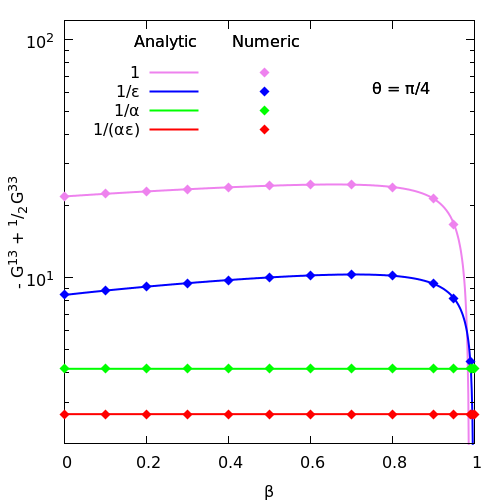
\includegraphics[width=0.45\textwidth]{../../vp-terms/plots/bubble-beta13.png}
 \hfill
 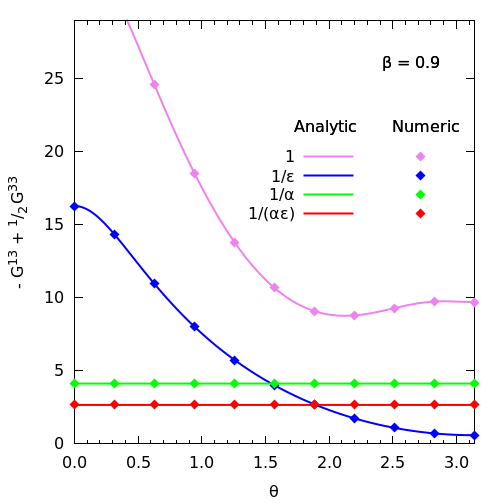
\includegraphics[width=0.45\textwidth]{../../vp-terms/plots/bubble-theta13.png}
 \end{center}
 \caption{
 Comparison of numeric and analytic results for example graphs contributing to
 the $n_f$ part of the NNLO soft function.
 }
 \label{fig:compG13}
\end{figure}


The above results provide strong checks of our framework. We were, however, able
to validate it further by comparing the numerical results for combinations of
quark-bubble graphs, obtained with the sector decomposition-based method, and
the analytic results from the method of differential equations. An example
comparison is presented in Fig.~\ref{fig:compG13} where the points (lines)
correspond to numeric (analytic) coefficients of different powers in the
expansion in $\alpha$ and $\epsilon$. We observe per-mille-level agreement for
this and all the remaining graphs that contribute to the $n_f$ part of the NNLO
soft function.

Having done all the validations and cross checks, we are now in a position to
calculate the finite, $\LT$-independent part of the bare NNLO soft function.
By combining it with appropriate contributions coming from $\bfS^{(1)}_\bare$,
following Eq.~(\ref{eq:renS2}),
we obtain the renormalized soft function, which, in the $q\bar q$ channel and
for a specific phase-space point, reads
%
\begin{equation}
  S^{(2),\text{ren}}_{q\bar q} 
  \left(\beta = \frac{2}{5}, \theta = \frac{\pi}{4}\right) =  
  \left(
    \begin{array}{cc}
        198.682  & -8.73644 \\
        -8.73644 &  211.739
    \end{array}
  \right)
  +
  i \left(
    \begin{array}{cc}
        0        &  23.0178  \\
        23.0178  &  0 
    \end{array}
  \right)\,.
  %\label{eq:}
\end{equation}
%
For more results, we refer the reader to Ref.~\cite{sfpaper}.

%-----------------------------------------------------------------------------
\section{Conclusions}

We presented the calculation of the complete, small-$q_T$ soft function for top
pair production at NNLO. In order to evaluate the most difficult divergent
integrals, originating from non-bubble, double cut diagrams, we developed a
framework based on sector decomposition. Other integrals were calculated either
directly, like in the case of single-cut diagrams, or by the method of
differential equations, which was applied to bubble integrals.
%
We performed a three-step validation of our results: by verifying that rapidity
singularities, and higher-order $\epsilon$ poles cancel, by cross-checking that
our direct calculation reproduces all terms predicted by the renormalization
group and, finally, by finding a perfect agreement between numeric results from
the sector decomposition-based framework and analytic results, for the graphs
involving gauge, ghost or quark bubble.
%
The NNLO, small-$q_T$ soft function  can now be used to obtain full $t\bar t$
cross section at NNLO by means of the $q_T$-slicing method, as well as for
small-$q_T$ resummation at NNLL'.


%-----------------------------------------------------------------------------
\section*{Acknowledgements}

This work has been supported by the National Science Centre, Poland grant
POLONEZ  
\begin{wrapfigure}[4]{r}{0.15\textwidth}
  \centering
  \vspace{-10pt}
  
\includegraphics[width=0.15\textwidth]{plots/flag_yellow_low.jpg}
\end{wrapfigure}
%
No. 2015/19/P/ST2/03007. 
%
The project has received funding from the
European Union's Horizon 2020 research  and  innovation  programme  under  the
Marie Sk\l{}odowska-Curie grant agreement No. 665778.
%
We are grateful to Mateusz Dobija for implementation of numerical integration
with CUBA.  

\begin{thebibliography}{99}

%\cite{Anastasiou:2015ema}
\bibitem{Anastasiou:2015ema}
  C.~Anastasiou, C.~Duhr, F.~Dulat, F.~Herzog and B.~Mistlberger,
  %``Higgs Boson Gluon-Fusion Production in QCD at Three Loops,''
  Phys.\ Rev.\ Lett.\  {\bf 114} (2015) 212001
  doi:10.1103/PhysRevLett.114.212001
  [arXiv:1503.06056 [hep-ph]].
  %%CITATION = doi:10.1103/PhysRevLett.114.212001;%%

%\cite{Baernreuther:2012ws}
\bibitem{Baernreuther:2012ws}
  P.~B\"arnreuther, M.~Czakon and A.~Mitov,
  %``Percent Level Precision Physics at the Tevatron: First Genuine NNLO QCD
  %Corrections to $q \bar{q} \to t \bar{t} + X$,''
  Phys.\ Rev.\ Lett.\  {\bf 109} (2012) 132001
  doi:10.1103/PhysRevLett.109.132001
  [arXiv:1204.5201 [hep-ph]].
  %%CITATION = doi:10.1103/PhysRevLett.109.132001;%%

%\cite{Czakon:2012pz}
\bibitem{Czakon:2012pz}
  M.~Czakon and A.~Mitov,
  %``NNLO corrections to top pair production at hadron colliders: the
  %quark-gluon reaction,''
  JHEP {\bf 1301} (2013) 080
  doi:10.1007/JHEP01(2013)080
  [arXiv:1210.6832 [hep-ph]].
  %%CITATION = doi:10.1007/JHEP01(2013)080;%%

%\cite{Czakon:2012zr}
\bibitem{Czakon:2012zr}
  M.~Czakon and A.~Mitov,
  %``NNLO corrections to top-pair production at hadron colliders: the
  %all-fermionic scattering channels,''
  JHEP {\bf 1212} (2012) 054
  doi:10.1007/JHEP12(2012)054
  [arXiv:1207.0236 [hep-ph]].
  %%CITATION = doi:10.1007/JHEP12(2012)054;%%

%\cite{Czakon:2013goa}
\bibitem{Czakon:2013goa}
  M.~Czakon, P.~Fiedler and A.~Mitov,
  %``Total Top-Quark Pair-Production Cross Section at Hadron Colliders Through
  %$O(α\frac{4}{S})$,''
  Phys.\ Rev.\ Lett.\  {\bf 110} (2013) 252004
  doi:10.1103/PhysRevLett.110.252004
  [arXiv:1303.6254 [hep-ph]].
  %%CITATION = doi:10.1103/PhysRevLett.110.252004;%%

%\cite{Czakon:2015owf}
\bibitem{Czakon:2015owf}
  M.~Czakon, D.~Heymes and A.~Mitov,
  %``High-precision differential predictions for top-quark pairs at the LHC,''
  Phys.\ Rev.\ Lett.\  {\bf 116} (2016) no.8,  082003
  doi:10.1103/PhysRevLett.116.082003
  [arXiv:1511.00549 [hep-ph]].
  %%CITATION = doi:10.1103/PhysRevLett.116.082003;%%

%\cite{Czakon:2016ckf}
\bibitem{Czakon:2016ckf}
  M.~Czakon, P.~Fiedler, D.~Heymes and A.~Mitov,
  %``NNLO QCD predictions for fully-differential top-quark pair production at
  %the Tevatron,''
  JHEP {\bf 1605} (2016) 034
  doi:10.1007/JHEP05(2016)034
  [arXiv:1601.05375 [hep-ph]].
  %%CITATION = doi:10.1007/JHEP05(2016)034;%%

%\cite{Catani:2007vq}
\bibitem{Catani:2007vq}
  S.~Catani and M.~Grazzini,
  %``An NNLO subtraction formalism in hadron collisions and its application to
  %Higgs boson production at the LHC,''
  Phys.\ Rev.\ Lett.\  {\bf 98} (2007) 222002
  doi:10.1103/PhysRevLett.98.222002
  [hep-ph/0703012].
  %%CITATION = doi:10.1103/PhysRevLett.98.222002;%%

%\cite{Bonciani:2015sha}
\bibitem{Bonciani:2015sha}
  R.~Bonciani, S.~Catani, M.~Grazzini, H.~Sargsyan and A.~Torre,
  %``The $q_T$ subtraction method for top quark production at hadron
  %colliders,''
  Eur.\ Phys.\ J.\ C {\bf 75} (2015) no.12,  581
  doi:10.1140/epjc/s10052-015-3793-y
  [arXiv:1508.03585 [hep-ph]].
  %%CITATION = doi:10.1140/epjc/s10052-015-3793-y;%%

%\cite{Becher:2014oda}
\bibitem{Becher:2014oda}
  T.~Becher, A.~Broggio and A.~Ferroglia,
  %``Introduction to Soft-Collinear Effective Theory,''
  Lect.\ Notes Phys.\  {\bf 896} (2015) pp.1
  doi:10.1007/978-3-319-14848-9
  [arXiv:1410.1892 [hep-ph]].
  %%CITATION = doi:10.1007/978-3-319-14848-9;%%

%\cite{Gehrmann:2012ze}
\bibitem{Gehrmann:2012ze}
  T.~Gehrmann, T.~Lubbert and L.~L.~Yang,
  %``Transverse parton distribution functions at next-to-next-to-leading order:
  %the quark-to-quark case,''
  Phys.\ Rev.\ Lett.\  {\bf 109} (2012) 242003
  doi:10.1103/PhysRevLett.109.242003
  [arXiv:1209.0682 [hep-ph]].
  %%CITATION = doi:10.1103/PhysRevLett.109.242003;%%

%\cite{Gehrmann:2014yya}
\bibitem{Gehrmann:2014yya}
  T.~Gehrmann, T.~Luebbert and L.~L.~Yang,
  %``Calculation of the transverse parton distribution functions at
  %next-to-next-to-leading order,''
  JHEP {\bf 1406} (2014) 155
  doi:10.1007/JHEP06(2014)155
  [arXiv:1403.6451 [hep-ph]].
  %%CITATION = doi:10.1007/JHEP06(2014)155;%%

%\cite{Czakon:2008zk}
\bibitem{Czakon:2008zk}
  M.~Czakon,
  %``Tops from Light Quarks: Full Mass Dependence at Two-Loops in QCD,''
  Phys.\ Lett.\ B {\bf 664} (2008) 307
  doi:10.1016/j.physletb.2008.05.028
  [arXiv:0803.1400 [hep-ph]].
  %%CITATION = doi:10.1016/j.physletb.2008.05.028;%%

%\cite{Baernreuther:2013caa}
\bibitem{Baernreuther:2013caa}
  P.~B\"arnreuther, M.~Czakon and P.~Fiedler,
  %``Virtual amplitudes and threshold behaviour of hadronic top-quark
  %pair-production cross sections,''
  JHEP {\bf 1402} (2014) 078
  doi:10.1007/JHEP02(2014)078
  [arXiv:1312.6279 [hep-ph]].
  %%CITATION = doi:10.1007/JHEP02(2014)078;%%

%\cite{Li:2013mia}
\bibitem{Li:2013mia}
  H.~T.~Li, C.~S.~Li, D.~Y.~Shao, L.~L.~Yang and H.~X.~Zhu,
  %``Top quark pair production at small transverse momentum in hadronic
  %collisions,''
  Phys.\ Rev.\ D {\bf 88} (2013) 074004
  doi:10.1103/PhysRevD.88.074004
  [arXiv:1307.2464 [hep-ph]].
  %%CITATION = doi:10.1103/PhysRevD.88.074004;%%

%\cite{Catani:2014qha}
\bibitem{Catani:2014qha}
  S.~Catani, M.~Grazzini and A.~Torre,
  %``Transverse-momentum resummation for heavy-quark hadroproduction,''
  Nucl.\ Phys.\ B {\bf 890} (2014) 518
  doi:10.1016/j.nuclphysb.2014.11.019
  [arXiv:1408.4564 [hep-ph]].
  %%CITATION = doi:10.1016/j.nuclphysb.2014.11.019;%%

\bibitem{Ferroglia:2012uy}
  A.~Ferroglia, B.~D.~Pecjak, L.~L.~Yang, B.~D.~Pecjak and L.~L.~Yang,
  %``The NNLO soft function for the pair invariant mass distribution of boosted
  %top quarks,''
  JHEP {\bf 1210} (2012) 180
  doi:10.1007/JHEP10(2012)180
  [arXiv:1207.4798 [hep-ph]].
  %%CITATION = doi:10.1007/JHEP10(2012)180;%%

\bibitem{Wang:2018vgu}
  G.~Wang, X.~Xu, L.~L.~Yang and H.~X.~Zhu,
  %``The next-to-next-to-leading order soft function for top quark pair
  %production,''
  JHEP {\bf 1806} (2018) 013
  doi:10.1007/JHEP06(2018)013
  [arXiv:1804.05218 [hep-ph]].
  %%CITATION = doi:10.1007/JHEP06(2018)013;%%

%\cite{Becher:2011dz}
\bibitem{Becher:2011dz}
  T.~Becher and G.~Bell,
  %``Analytic Regularization in Soft-Collinear Effective Theory,''
  Phys.\ Lett.\ B {\bf 713} (2012) 41
  doi:10.1016/j.physletb.2012.05.016
  [arXiv:1112.3907 [hep-ph]].
  %%CITATION = doi:10.1016/j.physletb.2012.05.016;%%

\bibitem{Zhu:2012ts}
  H.~X.~Zhu, C.~S.~Li, H.~T.~Li, D.~Y.~Shao and L.~L.~Yang,
  %``Transverse-momentum resummation for top-quark pairs at hadron colliders,''
  Phys.\ Rev.\ Lett.\  {\bf 110} (2013) no.8,  082001
  doi:10.1103/PhysRevLett.110.082001
  [arXiv:1208.5774 [hep-ph]].
  %%CITATION = doi:10.1103/PhysRevLett.110.082001;%%
  %40 citations counted in INSPIRE as of 13 Jul 2018

%\cite{Ahrens:2010zv}
\bibitem{Ahrens:2010zv}
  V.~Ahrens, A.~Ferroglia, M.~Neubert, B.~D.~Pecjak and L.~L.~Yang,
  %``Renormalization-Group Improved Predictions for Top-Quark Pair Production at
  %Hadron Colliders,''
  JHEP {\bf 1009} (2010) 097
  doi:10.1007/JHEP09(2010)097
  [arXiv:1003.5827 [hep-ph]].
  %%CITATION = doi:10.1007/JHEP09(2010)097;%%

%\cite{Becher:2010tm}
\bibitem{Becher:2010tm}
  T.~Becher and M.~Neubert,
  %``{Drell-Yan} Production at Small $q_T$, Transverse Parton Distributions and
  %the Collinear Anomaly,''
  Eur.\ Phys.\ J.\ C {\bf 71} (2011) 1665
  doi:10.1140/epjc/s10052-011-1665-7
  [arXiv:1007.4005 [hep-ph]].
  %%CITATION = doi:10.1140/epjc/s10052-011-1665-7;%%

%\cite{Becher:2012yn}
\bibitem{Becher:2012yn}
  T.~Becher, M.~Neubert and D.~Wilhelm,
  %``Higgs-Boson Production at Small Transverse Momentum,''
  JHEP {\bf 1305} (2013) 110
  doi:10.1007/JHEP05(2013)110
  [arXiv:1212.2621 [hep-ph]].
  %%CITATION = doi:10.1007/JHEP05(2013)110;%%

\bibitem{Laporta:2001dd}
  S.~Laporta,
  %``High precision calculation of multiloop Feynman integrals by difference
  %equations,''
  Int.\ J.\ Mod.\ Phys.\ A {\bf 15} (2000) 5087
  doi:10.1016/S0217-751X(00)00215-7, 10.1142/S0217751X00002157
  [hep-ph/0102033].
  %%CITATION = doi:10.1016/S0217-751X(00)00215-7, 10.1142/S0217751X00002157;%%

\bibitem{Ruijl:2017dtg}
  B.~Ruijl, T.~Ueda and J.~Vermaseren,
  %``FORM version 4.2,''
  arXiv:1707.06453 [hep-ph].
  %%CITATION = ARXIV:1707.06453;%%

\bibitem{fermat}
  R.~H.~Lewis,
  {\it Computer Algebra System} {\tt Fermat},
  {http://home.bway.net/lewis} .

%\cite{Binoth:2000ps}
\bibitem{Binoth:2000ps}
  T.~Binoth and G.~Heinrich,
  %``An automatized algorithm to compute infrared divergent multiloop
  %integrals,''
  Nucl.\ Phys.\ B {\bf 585} (2000) 741
  doi:10.1016/S0550-3213(00)00429-6
  [hep-ph/0004013].
  %%CITATION = doi:10.1016/S0550-3213(00)00429-6;%%

\bibitem{Binoth:2003ak}
  T.~Binoth and G.~Heinrich,
  %``Numerical evaluation of multiloop integrals by sector decomposition,''
  Nucl.\ Phys.\ B {\bf 680} (2004) 375
  doi:10.1016/j.nuclphysb.2003.12.023
  [hep-ph/0305234].
  %%CITATION = doi:10.1016/j.nuclphysb.2003.12.023;%%

%\cite{Hahn:2004fe}
\bibitem{Hahn:2004fe}
  T.~Hahn,
  %``CUBA: A Library for multidimensional numerical integration,''
  Comput.\ Phys.\ Commun.\  {\bf 168} (2005) 78
  doi:10.1016/j.cpc.2005.01.010
  [hep-ph/0404043].
  %%CITATION = doi:10.1016/j.cpc.2005.01.010;%%

\bibitem{sfpaper}
  R.~\'Angeles-Mart\'inez, M.~Czakon, S. Sapeta,
  to appear.

\end{thebibliography}

\end{document}
